%%%%%%%%%%%%%%%%%%%%%%%%%%%%%%%%%%%%%%%%%
% Journal Article
% LaTeX Template
% Version 1.4 (15/5/16)
%
% This template has been downloaded from:
% http://www.LaTeXTemplates.com
%
% Original author:
% Frits Wenneker (http://www.howtotex.com) with extensive modifications by
% Vel (vel@LaTeXTemplates.com)
%
% License:
% CC BY-NC-SA 3.0 (http://creativecommons.org/licenses/by-nc-sa/3.0/)
%
%%%%%%%%%%%%%%%%%%%%%%%%%%%%%%%%%%%%%%%%%

%----------------------------------------------------------------------------------------
%	PACKAGES AND OTHER DOCUMENT CONFIGURATIONS
%----------------------------------------------------------------------------------------

\documentclass[oneside,twocolumn]{article}

\usepackage{blindtext} % Package to generate dummy text throughout this template 

\usepackage{graphicx} % FKM: for figures
\usepackage{color} % FKM: for colored text
\usepackage{float} % FKM: for forcing figure placement

\usepackage[sc]{mathpazo} % Use the Palatino font
\usepackage[T1]{fontenc} % Use 8-bit encoding that has 256 glyphs
\linespread{1.05} % Line spacing - Palatino needs more space between lines
\usepackage{microtype} % Slightly tweak font spacing for aestheticsgins
\usepackage[small,labelfont=bf,up,up]{caption} % Custom captions under/above floats in tables or figures
\usepackage{booktabs} % Horizontal rules in tables
\usepackage{amsmath} % Text in equations

\usepackage{enumitem} % Customized lists
\setlist[itemize]{noitemsep} % Make itemize lists more compact

\usepackage{abstract} % Allows abstract customization
\renewcommand{\abstractnamefont}{\normalfont\bfseries} % Set the "Abstract" text to bold
\renewcommand{\abstracttextfont}{\normalfont\small\itshape} % Set the abstract itself to small italic text

\usepackage{titlesec} % Allows customization of titles

\usepackage{fancyhdr} % Headers and footers
\pagestyle{fancy} % All pages have headers and footers
\fancyhead{} % Blank out the default header
\fancyfoot{} % Blank out the default footer
\fancyhead[C]{Authors et al. $\bullet$ August 2018 $\bullet$ bio{\color{red}R}$\chi$ve} % Custom header text
\fancyfoot[RO,LE]{\thepage} % Custom footer text

\usepackage{titling} % Customizing the title section

\usepackage[hidelinks]{hyperref} % For hyperlinks in the PDF

\usepackage{natbib}

\setlength\columnsep{20pt}

%----------------------------------------------------------------------------------------
%	TITLE SECTION
%----------------------------------------------------------------------------------------

\setlength{\droptitle}{-4\baselineskip} % Move the title up

\pretitle{\begin{center}\Huge\bfseries} % Article title formatting
\posttitle{\end{center}} % Article title closing formatting
\title{How you should validate your probabilistic model implementation} % Article title
\author{\textsc{An author here$^{1*}$}, \textsc{Another author
    here$^{1*}$}, \textsc{Yet another author here$^{1*}$}, \\
  \textsc{Last author here$^{1*}$} \\
\small $^1$School of Computer Science, The University of Auckland\\
\small $^2$Department of Biology, The University of Auckland\\
\small \href{mailto:@aucklanduni.ac.nz}{$^*$@aucklanduni.ac.nz}
%\and % Uncomment if 2 authors are required, duplicate these 4 lines if more
%\textsc{Jane Smith}\thanks{Corresponding author} \\[1ex] % Second author's name
%\normalsize University of Utah \\ % Second author's institution
%\normalsize \href{mailto:jane@smith.com}{jane@smith.com} % Second author's email address
}
\date{\today} % Leave empty to omit a date
\renewcommand{\maketitlehookd}{%
\begin{abstract}
  \noindent \blindtext
\end{abstract}
}

%----------------------------------------------------------------------------------------

\begin{document}

% Print the title
\maketitle

%----------------------------------------------------------------------------------------
%	ARTICLE CONTENTS
%----------------------------------------------------------------------------------------

\section*{Introduction}
The last two decades have seen the biological sciences undergo a major revolution.
Critical technological innovations such as the advent of massive parallel sequencing and the accompanying improvements in computational power and storage have flooded biology with unprecedented amounts of data ripe for analysis.
Not only has intraspecific data from multiple individuals allowed
progress in disparate fields like medicine and epidemiology
\citep[e.g.,][]{1000g,humanmicrobiome,neafsey15}, population genetics \citep[e.g.,][]{lynch07,lack16,demanuel16} and disease ecology \citep[e.g.][]{rosenblum13,bates18}, but now a large number of species across the tree of life have had their genomes sequenced, furthering our understanding of species relationships and diversification \citep[e.g.,][]{Martin_Genome_2013,brawand14,jarvis14,novikova16,Pease2016}.
However, as the old adage goes, with great power comes great responsibility: never has the data available to the average biologist been so abundant, but also never has one been so aware of both its complexity and the necessary care with which to analyze it.
Almost at par with with data accumulation is the rate at which new computational tools are being proposed, as evidenced by journals entirely dedicated to method advances, methodological sections in biological journals, and computational biology degrees being offered by institutions around the world.

One extreme case is the discipline of evolutionary biology (on which we focus our attention).
While it could be said that many decade-old questions and hypotheses
in evolutionary biology have aged well and stood up the test of time
(e.g., the Red Queen hypothesis,
\citealt{vanvalen73,lively87,morran11,gibson15}; the
Bateson-Dobzhansky-Muller model, \citealt{dob36,muller40,hopkins12,roda17}), data analysis
practices have changed drastically in recent years (Fig. 1), to the
point they would likely seem obscure to an evolutionary biologist last active 40 years ago.
In particular, evolutionary biology has become highly statistical, with the development and utilization of models now being commonplace.

Models are employed in the sciences for many reasons, and fall within
a biological abstraction continuum \citep{servedio14}, going from
fully verbal, highly abstract models (e.g., \citealt{vanvalen73}), through proof-of-concept models
that formalize verbal models (e.g., \citealt{maynard78,reinhold99,mendes18}), to probabilistic models that interact
directly with data (i.e., models with a likelihood function such as \citealt{yule24,felsenstein73,hky,hudson90}).
Though mathematical models are in general more frequently used in
evolutionary biology, there has been a sharp surge in instances of the
latter cases (i.e., probabilistic models) in conjunction with computational tools implementing them
(Fig. 1).

\vspace{.5cm}

\noindent [Say something about how validation is overlooked/underappreciated; by
users, who use packages blindly; by developers, who don't make their
unit tests readily available or visible, despite open source code; by reviewers, who don't
demand stringent tests]

Here, we summarize best practices in probabilistic  model validation for method
developers, with an emphasis on Bayesian methods.
We also introduce a new BEAST 2 package, \texttt{THE SWANEPOEL}, which
provides tests that newly implemented likelihood classes can
be subjected to.
We hope our guidelines can help raise the standards for software
package releases required by users, developers and reviewers alike,
and consequently lead to computational tools that are more efficient, better documented, and most
importantly, correctly implemented.

% \begin{figure}
%   \includegraphics[width=\linewidth]{fig1}
%   \caption{Hemiplasy on species trees and gene trees.
%     Panel (a) shows substitutions that occur on each of the two discordant gene trees, and the corresponding site patterns produced.
%     (b) Incorrectly inferred convergent substitutions (from the site patterns produced in [a]) when analyses are conducted on the species tree topology.
%     (c) Incorrectly inferred convergent substitutions when analyses are conducted on the CDS tree (discordant tree topology 2).}
%   \label{fig:1}
% \end{figure}

%------------------------------------------------

\section*{Probabilistic model validation}
\subsection*{Verifying the correctness of a model's likelihood}

The central component of a probabilistic model is its likelihood
function, $P(D|\theta)$, which establishes the
interface between an abstract representation of reality (defined by parameters $\theta$), and the
empirical world (from which data $D$ is obtained).
In a frequentist statistical framework, the likelihood function is the sole
component of a probabilistic model.
Here, tasks like parameter estimation and model comparison are conducted
by maximizing the likelihood function across parameter
space.

In Bayesian inference, on the other hand, a probabilistic model
defines a posterior probability distribution for its parameters,
$P(\theta|D) = P(\theta|D)P(\theta) / P(D)$, in which our prior
knowledge or beliefs about the natural world -- represented by the prior
distribution $P(\theta)$ -- are confronted and updated by the data through the
likelihood function.
$P(D) = \int_\theta P(D|\theta)P(\theta)d\theta$, the probability of
the data, is also known as the marginal likelihood or the model evidence.
Under simple-enough models, the probability density function of the posterior distribution can sometimes be analytically
derived.
Models routinely used in biology are nonetheless often complex enough
to preclude such closed-form solutions, mainly due to the
intractability of the integral that appears in the marginal
likelihood.
In those cases, techniques like Markov Chain Monte Carlo (MCMC) can be employed to
sample the posterior distribution (but see \citealt{zhang18}).
When MCMC is conducted, one can use the fact that $P(D)$
evaluates to a constant that can be conveniently ignored, i.e., $P(\theta|D) \propto P(\theta|D)P(\theta)$.

A good starting point when validating the implementation of a probabilistic
model is the comparison between the value of its likelihood function given
specific parameter values to some expected value $z$, that
is, evaluating $P(D|\theta)$ for some $\theta$, and comparing the
result to $z$.
What should $z$ be? When models are sufficiently simple, or by focusing
on a subcase of a complex model, it is often straightforward to derive
what $z$ should be.

For example, one commonly used model in macroevolution, specifically in the study
of continuous trait evolution, is a random walk model known as
Brownian motion (BM; \citealt{felsenstein73}).
The log-likelihood function of this model is simply the multivariate
normal probability density function:

\begin{equation}
  \begin{split}
    \text{log P}(\mathbf{y} \mid \mathbf{y_0}, r, \mathbf{T}) = -\frac{1}{2} \Big[ n\text{log}(2\pi) + \text{log}|r \mathbf{T}| \Big] & \\
    -\frac{1}{2} \Big[ (\mathbf{y} - \mathbf{y_0})^T (r \mathbf{T})^{-1} (\mathbf{y} - \mathbf{y_0}) \Big],
  \label{eq:1}
  \end{split}
\end{equation}

\noindent where $\mathbf{y}$ corresponds to the mean trait values in $n$ species,
$y_0$ is the trait value at the root, $r$ is the variance of the process
(also known as the evolutionary rate, and sometimes represented by $\sigma^2$), and $\mathbf{T}$ is the
variance-covariance matrix derived from the species tree.
Following the notation from before, under this model $\theta = \{y_0,
r\}$ and $D = \{\mathbf{y, \mathbf{T}} \}$ (but note that $\mathbf{T}$ can
be a parameter elsewhere in a hierarchical model of which BM is just a
component).
For a small tree -- e.g., (A:1.0,B:1.0) -- the likelihood of a given set
of parameter values $\theta$ can be computed with pen and paper and compared to
the output of a focal implementation.

While this is a very trivial validation procedure, it is a crucial first
step for more complex tests, and of particular use to likelihood functions that can be
implemented with different algorithms.
The likelihood of the BM model, for example, can be computed using a
dynamic-programming algorithm known in the phylogenetics literature
as the ``pruning'' or ``peeling'' algorithm \citep{felsenstein73}.
If a BM model is implemented correctly, the likelihood of any specific
$\theta$ should match the solution of equation \ref{eq:1} no matter which algorithm is used.

More thorough correctness checks occur when $z$ can be
compared to a quantity that emerges from a valid model implementation,
rather than to the likelihood value itself.
One such instance is the well-established Kingman's coalescent model \citep{kingman82}
from population genetics, the likelihood function of which is given by:

\begin{equation}
  P(T \mid N_e) = \prod_{k=2}^{n} \Bigg( \frac{1}{N_e} \text{exp} \Bigg(
  \frac{k(k-1)t_k}{2N_e} \Bigg) \Bigg),
  \label{eq:2}
\end{equation}

\noindent where $n$ is the number of lineages we sampled, $t_k$ is the time during which $k$ lineages
coexist, and $N_e$ is the effective population size.
Here, the data is a genealogy $T$ that defines a set of intervals
between coalescence events.
Interestingly, while the height of $T$, $T_{MRCA}$ (the time to the most
recent common ancestor of all $n$ samples), is not part of the
likelihood function, it can be derived from the properties of the
model:

\begin{equation}
  \text{E}[T_{MRCA}] = 2 \bigg(1-\frac{1}{n}\bigg),
  \label{eq:3}
\end{equation}

\noindent \citep{hudson90}.
One way to verify the correctness of an implementation of the Kingman's
coalescent, for example, is then to simulate genealogies given some
$N_e$ and compare the genalogical heights with the result of equation
\ref{eq:3}.
In a Bayesian framework this procedure amounts to a direct validation of the
likelihood if one carries out MCMC without any data (i.e., sampling
from the prior), but also to a validation of all the machinery involved in MCMC.

Alternatively, when theoretical expectations cannot be derived from
the model itself, usually due to complexity of its formulation, {\color{red}{[Place holder for Christiaan's text]}}

Finally, whether or not theoretical expectations can be
derived, one can generate expectations from independent (validated) model implementations.
If such implementations are available, likelihood values or other
quantities can be promptly computed or simulated and compared against.

\subsection*{Bayesian model validation}

[Validating operators]

\vspace{1cm}

\noindent [Coverage]

\begin{figure}
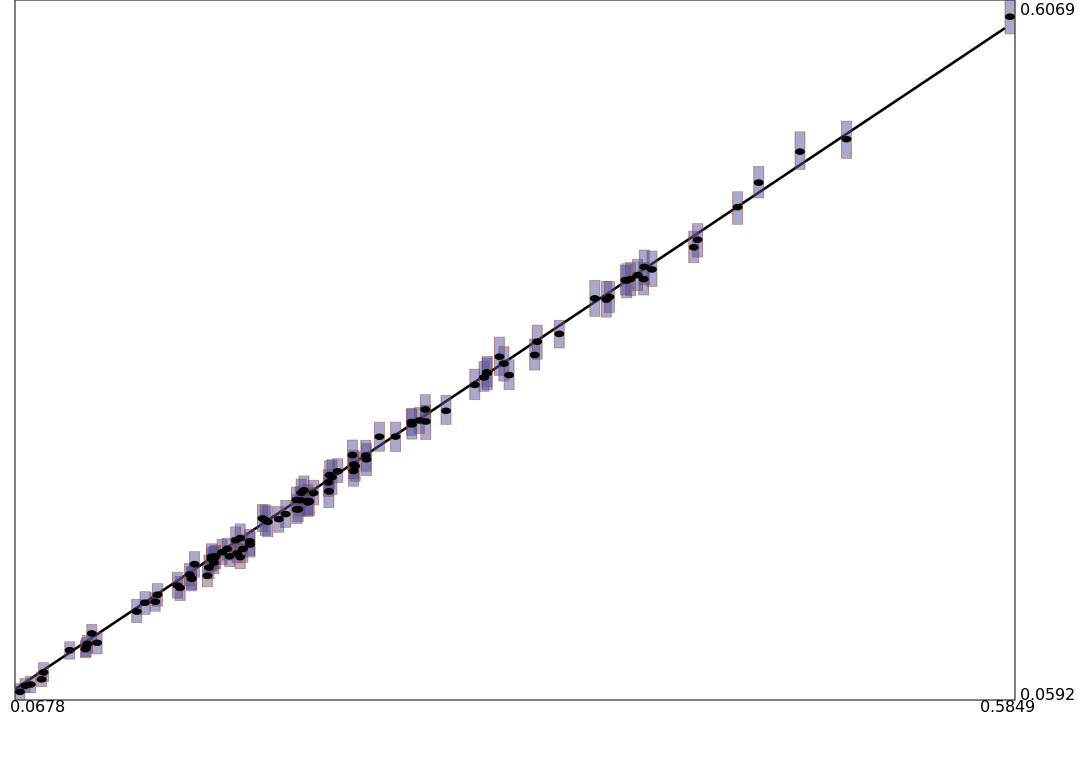
\includegraphics[width=0.19\textwidth]{../figures/bargraph-ok-strong}
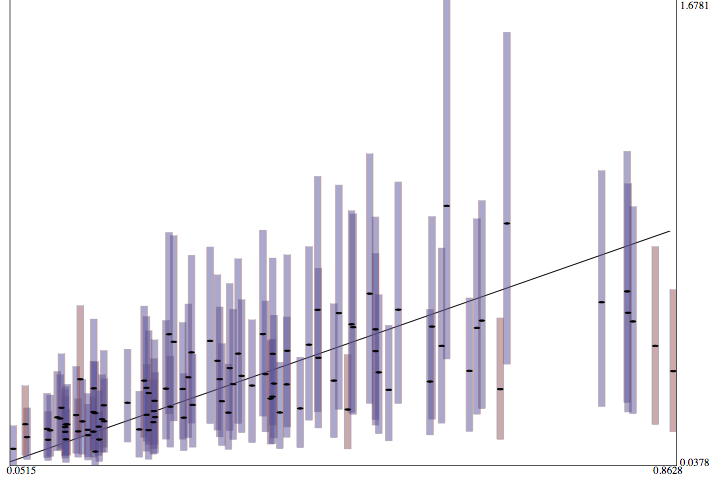
\includegraphics[width=0.19\textwidth]{../figures/bargraph-ok-medium}
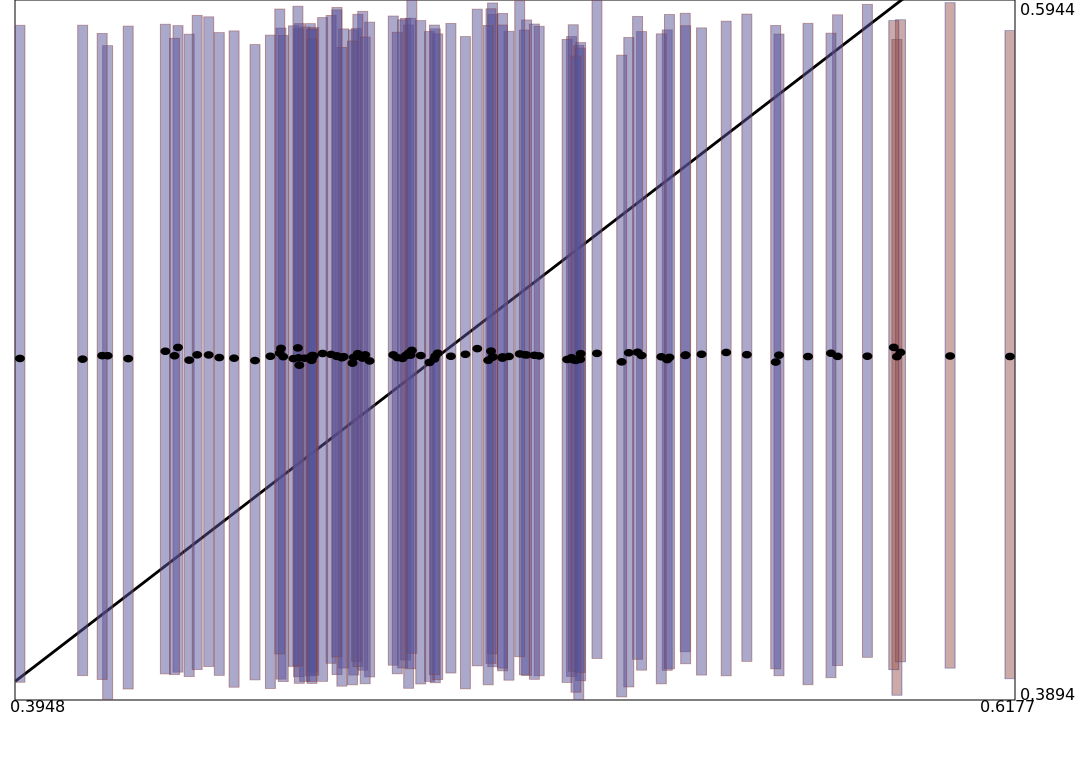
\includegraphics[width=0.19\textwidth]{../figures/bargraph-ok-weak}
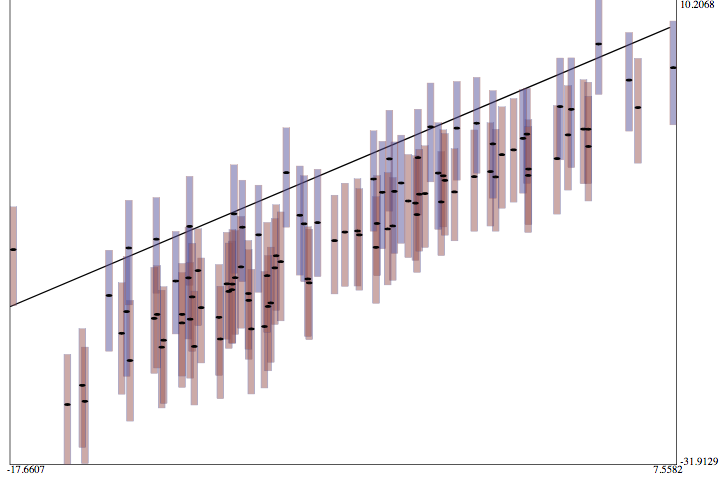
\includegraphics[width=0.19\textwidth]{../figures/bargraph-under}
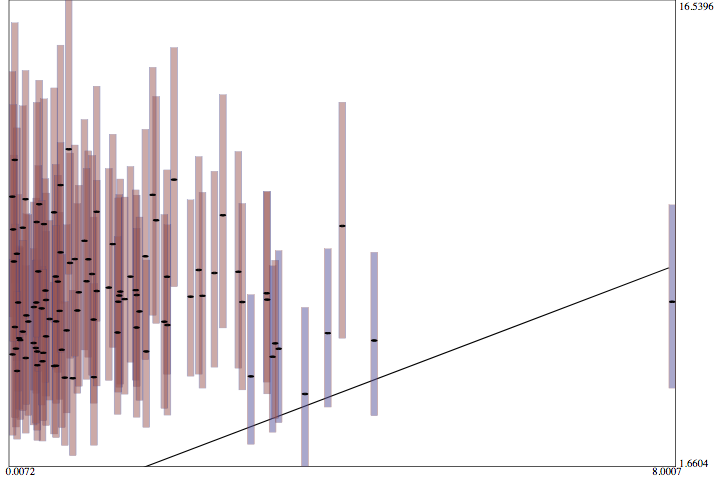
\includegraphics[width=0.19\textwidth]{../figures/bargraph-over}
\caption{\label{fig:coverage}
Graphs show true value on x-axis and estimates on y-axis. Black line shows where x equals y axis, and where ideally most of the probability mass is concentrated. Black dots are means of estimates. Bars indicate 95\% HPDs where blue bars cover the true value and red ones do not. Ideally 95 out of 100 bars should be blue.
a) Strong coverage: true parameter can be inferred accurately.
b) Medium coverage: true parameter can be inferred, but with high uncertainty.
c) Weak coverage: true parameter cannot be inferred, even though 95\% HPD covers the true value sufficiently often.
d) True parameter is over estimated.
e) True parameter is under estimated.
}
\end{figure}


\vspace{1cm}

\noindent [Well-calibrated validation: coverage, correlation between truth and
mean posteriors]

\vspace{1cm}

\noindent [Table: Bayesian packages that have (or not) done well-calibrated
validation studies]

\section*{Concluding remarks}
Blabla

\subsection*{Authors' contributions}
Blabla

\subsection*{Funding}
Blabla


%----------------------------------------------------------------------------------------
%	REFERENCE LIST
%----------------------------------------------------------------------------------------

% \section*{References}
% \clearpage

\bibliographystyle{sysbio}
\bibliography{refs}

%----------------------------------------------------------------------------------------

\end{document}
